% Options for packages loaded elsewhere
% Options for packages loaded elsewhere
\PassOptionsToPackage{unicode}{hyperref}
\PassOptionsToPackage{hyphens}{url}
%
\documentclass[
  ignorenonframetext,
]{beamer}
\newif\ifbibliography
\usepackage{pgfpages}
\setbeamertemplate{caption}[numbered]
\setbeamertemplate{caption label separator}{: }
\setbeamercolor{caption name}{fg=normal text.fg}
\beamertemplatenavigationsymbolsempty
% remove section numbering
\setbeamertemplate{part page}{
  \centering
  \begin{beamercolorbox}[sep=16pt,center]{part title}
    \usebeamerfont{part title}\insertpart\par
  \end{beamercolorbox}
}
\setbeamertemplate{section page}{
  \centering
  \begin{beamercolorbox}[sep=12pt,center]{section title}
    \usebeamerfont{section title}\insertsection\par
  \end{beamercolorbox}
}
\setbeamertemplate{subsection page}{
  \centering
  \begin{beamercolorbox}[sep=8pt,center]{subsection title}
    \usebeamerfont{subsection title}\insertsubsection\par
  \end{beamercolorbox}
}
% Prevent slide breaks in the middle of a paragraph
\widowpenalties 1 10000
\raggedbottom
\AtBeginPart{
  \frame{\partpage}
}
\AtBeginSection{
  \ifbibliography
  \else
    \frame{\sectionpage}
  \fi
}
\AtBeginSubsection{
  \frame{\subsectionpage}
}
\usepackage{iftex}
\ifPDFTeX
  \usepackage[T1]{fontenc}
  \usepackage[utf8]{inputenc}
  \usepackage{textcomp} % provide euro and other symbols
\else % if luatex or xetex
  \usepackage{unicode-math} % this also loads fontspec
  \defaultfontfeatures{Scale=MatchLowercase}
  \defaultfontfeatures[\rmfamily]{Ligatures=TeX,Scale=1}
\fi
\usepackage{lmodern}

\usetheme[]{style.scss}
\ifPDFTeX\else
  % xetex/luatex font selection
\fi
% Use upquote if available, for straight quotes in verbatim environments
\IfFileExists{upquote.sty}{\usepackage{upquote}}{}
\IfFileExists{microtype.sty}{% use microtype if available
  \usepackage[]{microtype}
  \UseMicrotypeSet[protrusion]{basicmath} % disable protrusion for tt fonts
}{}
\makeatletter
\@ifundefined{KOMAClassName}{% if non-KOMA class
  \IfFileExists{parskip.sty}{%
    \usepackage{parskip}
  }{% else
    \setlength{\parindent}{0pt}
    \setlength{\parskip}{6pt plus 2pt minus 1pt}}
}{% if KOMA class
  \KOMAoptions{parskip=half}}
\makeatother


\usepackage{longtable,booktabs,array}
\usepackage{calc} % for calculating minipage widths
\usepackage{caption}
% Make caption package work with longtable
\makeatletter
\def\fnum@table{\tablename~\thetable}
\makeatother
\usepackage{graphicx}
\makeatletter
\newsavebox\pandoc@box
\newcommand*\pandocbounded[1]{% scales image to fit in text height/width
  \sbox\pandoc@box{#1}%
  \Gscale@div\@tempa{\textheight}{\dimexpr\ht\pandoc@box+\dp\pandoc@box\relax}%
  \Gscale@div\@tempb{\linewidth}{\wd\pandoc@box}%
  \ifdim\@tempb\p@<\@tempa\p@\let\@tempa\@tempb\fi% select the smaller of both
  \ifdim\@tempa\p@<\p@\scalebox{\@tempa}{\usebox\pandoc@box}%
  \else\usebox{\pandoc@box}%
  \fi%
}
% Set default figure placement to htbp
\def\fps@figure{htbp}
\makeatother





\setlength{\emergencystretch}{3em} % prevent overfull lines

\providecommand{\tightlist}{%
  \setlength{\itemsep}{0pt}\setlength{\parskip}{0pt}}



 


<link rel = "shortcut icon" href = "./figures/question_book.png" />
\makeatletter
\@ifpackageloaded{caption}{}{\usepackage{caption}}
\AtBeginDocument{%
\ifdefined\contentsname
  \renewcommand*\contentsname{Table of contents}
\else
  \newcommand\contentsname{Table of contents}
\fi
\ifdefined\listfigurename
  \renewcommand*\listfigurename{List of Figures}
\else
  \newcommand\listfigurename{List of Figures}
\fi
\ifdefined\listtablename
  \renewcommand*\listtablename{List of Tables}
\else
  \newcommand\listtablename{List of Tables}
\fi
\ifdefined\figurename
  \renewcommand*\figurename{Figure}
\else
  \newcommand\figurename{Figure}
\fi
\ifdefined\tablename
  \renewcommand*\tablename{Table}
\else
  \newcommand\tablename{Table}
\fi
}
\@ifpackageloaded{float}{}{\usepackage{float}}
\floatstyle{ruled}
\@ifundefined{c@chapter}{\newfloat{codelisting}{h}{lop}}{\newfloat{codelisting}{h}{lop}[chapter]}
\floatname{codelisting}{Listing}
\newcommand*\listoflistings{\listof{codelisting}{List of Listings}}
\makeatother
\makeatletter
\makeatother
\makeatletter
\@ifpackageloaded{caption}{}{\usepackage{caption}}
\@ifpackageloaded{subcaption}{}{\usepackage{subcaption}}
\makeatother

\usepackage{bookmark}
\IfFileExists{xurl.sty}{\usepackage{xurl}}{} % add URL line breaks if available
\urlstyle{same}
\hypersetup{
  hidelinks,
  pdfcreator={LaTeX via pandoc}}



\author{}
\date{}
\logo{\includegraphics{figures/question\_book.png}}

\begin{document}


\begin{frame}{}
\phantomsection\label{section}
{Curious Archives}

or: Books that question you


\includegraphics[width=0.4\linewidth,height=\textheight,keepaspectratio]{./figures/question_book.png}
\end{frame}

\begin{frame}{Intro}
\phantomsection\label{intro}
\begin{columns}[T]
\begin{column}{0.6\linewidth}
\begin{itemize}
\tightlist
\item
  Matthew Gemmell (he/him)
\item
  Microbiology background
\item
  CGR (UoL) \& NEOF
\item
  ELIXIR-UK Training club committee
\item
  Bioinformatics trainer

  \begin{itemize}
  \tightlist
  \item
    Since 2015
  \item
    10-15 workshop p/a
  \item
    \textgreater{} 70 workshops
  \end{itemize}
\end{itemize}
\end{column}

\begin{column}{0.4\linewidth}
\pandocbounded{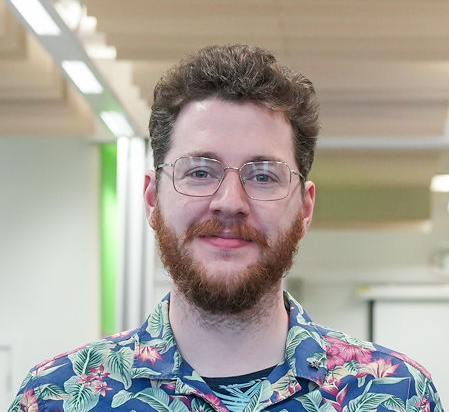
\includegraphics[keepaspectratio]{./figures/mg_headshot.png}}

\pandocbounded{
\includegraphics[keepaspectratio]{./figures/NEOF.png}}

\pandocbounded{
\includegraphics[keepaspectratio]{./figures/Full colour logo.png}}
\end{column}
\end{columns}
\end{frame}

\begin{frame}{Contents}
\phantomsection\label{contents}
\begin{columns}[T]
\begin{column}{0.6\linewidth}
\begin{itemize}
\item
  Formative assessment
\item
  MCQs

  \begin{itemize}
  \item
    Good practices
  \item
    Different uses
  \end{itemize}
\end{itemize}
\end{column}

\begin{column}{0.4\linewidth}

\includegraphics[width=1\linewidth,height=\textheight,keepaspectratio]{./figures/introduction.png}
\end{column}
\end{columns}
\end{frame}

\begin{frame}{}
\phantomsection\label{section-1}
{Formative Assessment}


\includegraphics[width=0.4\linewidth,height=\textheight,keepaspectratio]{./figures/formative_assessment.png}
\end{frame}

\begin{frame}{Formative assessment}
\phantomsection\label{formative-assessment}
\begin{columns}[T]
\begin{column}{0.6\linewidth}
\begin{itemize}
\tightlist
\item
  Continuous checks and balances during learning
\item
  Teacher checks:

  \begin{itemize}
  \tightlist
  \item
    Learner's progress
  \item
    Effectiveness of teaching practice
  \end{itemize}
\item
  Self assessment of learners
\item
  Very different to Summative assessment (e.g.~exams)
\end{itemize}
\end{column}

\begin{column}{0.4\linewidth}

\includegraphics[width=1\linewidth,height=\textheight,keepaspectratio]{./figures/formative_assessment.png}
\end{column}
\end{columns}
\end{frame}

\begin{frame}{Benefits}
\phantomsection\label{benefits}
\begin{columns}[T]
\begin{column}{0.75\linewidth}
\begin{itemize}
\tightlist
\item
  Be beneficial and enjoyable for students (Adkins, 2018)
\item
  Help students monitor their progress and encourage further study
  (McCallum \& Milner, 2021)
\item
  Incorporate aspects of a flipped classroom

  \begin{itemize}
  \tightlist
  \item
    Self paced
  \item
    Decrease cognitive load
  \item
    Support a diverse group of students in their learning
  \item
    (Cortese et al., 2022)
  \end{itemize}
\end{itemize}
\end{column}

\begin{column}{0.25\linewidth}

\includegraphics[width=1\linewidth,height=\textheight,keepaspectratio]{./figures/benefit.png}
\end{column}
\end{columns}
\end{frame}

\begin{frame}{Variety}
\phantomsection\label{variety}
\begin{columns}[T]
\begin{column}{0.7\linewidth}
\begin{itemize}
\tightlist
\item
  Formative assessment gives variety
\item
  Stop reading, start applying
\item
  Exercises

  \begin{itemize}
  \tightlist
  \item
    Include an answer chapter
  \end{itemize}
\item
  Verbally ask learners their progress and understanding
\item
  MCQs (Multiple Choice Questions)
\end{itemize}
\end{column}

\begin{column}{0.3\linewidth}

\includegraphics[width=1\linewidth,height=\textheight,keepaspectratio]{./figures/spices.png}
\end{column}
\end{columns}
\end{frame}

\begin{frame}{}
\phantomsection\label{section-2}
{MCQs}


\includegraphics[width=0.4\linewidth,height=\textheight,keepaspectratio]{./figures/quiz.png}
\end{frame}

\begin{frame}{MCQs}
\phantomsection\label{mcqs}
\begin{columns}[T]
\begin{column}{0.6\linewidth}
\begin{itemize}
\tightlist
\item
  Multiple Choice Question
\item
  Webexercises R package
\item
  Bookdown/Quarto
\end{itemize}

\begin{enumerate}
\tightlist
\item
  Question?
\end{enumerate}

\begin{itemize}
\tightlist
\item
  \begin{enumerate}
  [(A)]
  \tightlist
  \item
    \textbf{A1}\\
  \end{enumerate}
\item
  \begin{enumerate}
  [(A)]
  \setcounter{enumi}{1}
  \tightlist
  \item
    \textbf{A2}\\
  \end{enumerate}
\item
  \begin{enumerate}
  [(A)]
  \setcounter{enumi}{2}
  \tightlist
  \item
    \textbf{A3}
  \end{enumerate}
\end{itemize}
\end{column}

\begin{column}{0.4\linewidth}

\includegraphics[width=1\linewidth,height=\textheight,keepaspectratio]{./figures/quiz.pdf}
\end{column}
\end{columns}
\end{frame}

\begin{frame}{Bioinformatics (bfx)}
\phantomsection\label{bioinformatics-bfx}
\begin{columns}[T]
\begin{column}{0.7\linewidth}
\begin{itemize}
\tightlist
\item
  Multi disciplinary topic

  \begin{itemize}
  \tightlist
  \item
    Genomics, Computer science, \& Statistics
  \end{itemize}
\item
  2 main types of bfx learners

  \begin{itemize}
  \tightlist
  \item
    Life scientists
  \item
    Computational background
  \end{itemize}
\item
  I primarily teach life scientists

  \begin{itemize}
  \tightlist
  \item
    Assume basic level of biology
  \item
    Can't gain benefit of interaction with computational-based learners
  \end{itemize}
\end{itemize}
\end{column}

\begin{column}{0.3\linewidth}
\includegraphics[width=1\linewidth,height=\textheight,keepaspectratio]{./figures/seqio.png}
\end{column}
\end{columns}
\end{frame}

\begin{frame}{Master as a Service}
\phantomsection\label{master-as-a-service}
\begin{columns}[T]
\begin{column}{0.6\linewidth}
\begin{itemize}
\tightlist
\item
  Approach for multi disciplinary topics
\item
  Partner learners from different backgrounds
\item
  Initial reluctance by students
\item
  End point:

  \begin{itemize}
  \tightlist
  \item
    Students highly satisfied
  \item
    Benefited from learning skills and knowledge of students from other
    backgrounds
  \end{itemize}
\item
  (Navarro et al, 2019)
\end{itemize}
\end{column}

\begin{column}{0.4\linewidth}
\includegraphics[width=1\linewidth,height=\textheight,keepaspectratio]{./figures/multidisciplinary.png}
\end{column}
\end{columns}
\end{frame}

\begin{frame}{Working academic adults}
\phantomsection\label{working-academic-adults}
\begin{columns}[T]
\begin{column}{0.6\linewidth}
\begin{itemize}
\tightlist
\item
  PhD students, ECRs
\item
  Abundance of motivation

  \begin{itemize}
  \tightlist
  \item
    Want and/or need to learn (Taylor \& Hamdy, 2013)
  \item
    Know what they need to learn (Kara et al, 2019)
  \end{itemize}
\end{itemize}
\end{column}

\begin{column}{0.4\linewidth}
\includegraphics[width=1\linewidth,height=\textheight,keepaspectratio]{./figures/low_battery.png}
\end{column}
\end{columns}

\begin{itemize}
\tightlist
\item
  Low in time

  \begin{itemize}
  \tightlist
  \item
    Full time jobs, Household tasks, \& Caring responsibilities
    (children/dependants) (Cercone, 2008)
  \end{itemize}
\end{itemize}
\end{frame}

\begin{frame}{Case study}
\phantomsection\label{case-study}
\begin{columns}[T]
\begin{column}{0.6\linewidth}
\begin{itemize}
\item
  Literature review
\item
  Survey

  \begin{itemize}
  \tightlist
  \item
    Likert scaled questions
  \item
    Open questions
  \end{itemize}
\item
  Online courses
\item
  Synchronous and asynchronous
\item
  Engagement \& completion
\item
  Advantages and disadvantages
\end{itemize}
\end{column}

\begin{column}{0.4\linewidth}
\includegraphics[width=1\linewidth,height=\textheight,keepaspectratio]{./figures/case_study.png}
\end{column}
\end{columns}
\end{frame}

\begin{frame}{Survey}
\phantomsection\label{survey}
\begin{itemize}
\tightlist
\item
  Google form
\item
  Ethics disclaimer and collective ethics approval form
\item
  University of Liverpool staff (8 responses)
\end{itemize}

\pandocbounded{\includegraphics[keepaspectratio]{figures/career.png}}
\end{frame}

\begin{frame}{}
\phantomsection\label{section-3}
{Engagement and completion}


\includegraphics[width=0.4\linewidth,height=\textheight,keepaspectratio]{./figures/finish_flag.png}
\end{frame}

\begin{frame}{Course attendance and engagement}
\phantomsection\label{course-attendance-and-engagement}
\pandocbounded{\includegraphics[keepaspectratio]{figures/attendance.png}}

\pandocbounded{\includegraphics[keepaspectratio]{figures/engagement.png}}
\end{frame}

\begin{frame}{Breakdown}
\phantomsection\label{breakdown}
\begin{longtable}[]{@{}
  >{\centering\arraybackslash}p{(\linewidth - 6\tabcolsep) * \real{0.2424}}
  >{\centering\arraybackslash}p{(\linewidth - 6\tabcolsep) * \real{0.2500}}
  >{\centering\arraybackslash}p{(\linewidth - 6\tabcolsep) * \real{0.2424}}
  >{\centering\arraybackslash}p{(\linewidth - 6\tabcolsep) * \real{0.2500}}@{}}
\toprule\noalign{}
\begin{minipage}[b]{\linewidth}\centering
Synchronous course attendance
\end{minipage} & \begin{minipage}[b]{\linewidth}\centering
Asynchronous course attendance
\end{minipage} & \begin{minipage}[b]{\linewidth}\centering
Synchronous course engagement
\end{minipage} & \begin{minipage}[b]{\linewidth}\centering
Asynchronous course engagement
\end{minipage} \\
\midrule\noalign{}
\endhead
\textbf{1-2} & \textbf{1-2} & \textbf{4} & \textbf{4} \\
\textbf{1-2} & \textbf{1-2} & \textbf{4} & \textbf{2} \\
\textbf{1-2} & \textbf{1-2} & \textbf{4} & \textbf{2} \\
\textbf{1-2} & \textbf{1-2} & \textbf{2} & \textbf{4} \\
\textbf{3-5} & \textbf{3-5} & \textbf{5} & \textbf{3} \\
\textbf{1-2} & \textbf{1-2} & \textbf{4} & \textbf{4} \\
\textbf{1-2} & \textbf{1-2} & \textbf{5} & \textbf{4} \\
\textbf{5+} & \textbf{3-5} & \textbf{5} & \textbf{3} \\
\bottomrule\noalign{}
\end{longtable}
\end{frame}

\begin{frame}{Engagement}
\phantomsection\label{engagement}
\begin{columns}[T]
\begin{column}{0.6\linewidth}
\begin{itemize}
\tightlist
\item
  More likely to engage and complete synchronous courses
\item
  Dropouts are a crucial problem of adult learning (Park \& Choi, 2009,
  Choi \& Kim, 2018)
\item
  Studies have found limited engagement in pre-class materials in higher
  education (Al-Zahrani, 2015)
\end{itemize}
\end{column}

\begin{column}{0.4\linewidth}
\includegraphics[width=1\linewidth,height=\textheight,keepaspectratio]{./figures/engage.png}
\end{column}
\end{columns}
\end{frame}

\begin{frame}{}
\phantomsection\label{section-4}
{Synchronous courses}

\includegraphics[width=0.4\linewidth,height=\textheight,keepaspectratio]{./figures/synchronous_learning.png}
\end{frame}

\begin{frame}{Synchronous advantages}
\phantomsection\label{synchronous-advantages}
How beneficial do you find:

\pandocbounded{\includegraphics[keepaspectratio]{figures/sync_benefits.png}}
\end{frame}

\begin{frame}{Blocked out time}
\phantomsection\label{blocked-out-time}
\begin{columns}[T]
\begin{column}{0.6\linewidth}
\begin{itemize}
\tightlist
\item
  Response with highest perceived benefit
\item
  All responses extremely beneficial (bar one beneficial)
\item
  Easier to get break when event in calendar
\item
  Low time, especially:

  \begin{itemize}
  \tightlist
  \item
    middle-aged adults (36-55)
  \item
    female learners who are married and have children
  \item
    (Selwyn, 2011, Kara et al, 2019)
  \end{itemize}
\end{itemize}
\end{column}

\begin{column}{0.4\linewidth}
\includegraphics[width=1\linewidth,height=\textheight,keepaspectratio]{./figures/calender.png}
\end{column}
\end{columns}
\end{frame}

\begin{frame}{Synchronous advantages}
\phantomsection\label{synchronous-advantages-1}
How beneficial do you find:

\pandocbounded{\includegraphics[keepaspectratio]{figures/sync_benefits.png}}
\end{frame}

\begin{frame}{Learner-learner interaction}
\phantomsection\label{learner-learner-interaction}
\begin{columns}[T]
\begin{column}{0.6\linewidth}
\begin{itemize}
\tightlist
\item
  Mixed response

  \begin{itemize}
  \tightlist
  \item
    5 beneficial
  \item
    3 unbeneficial
  \item
    No neutrals
  \end{itemize}
\item
  Discussion with fellow learners

  \begin{itemize}
  \tightlist
  \item
    Share struggles and solutions
  \end{itemize}
\item
  Distraction from course

  \begin{itemize}
  \tightlist
  \item
    Zoom quiet room
  \end{itemize}
\end{itemize}
\end{column}

\begin{column}{0.4\linewidth}
\includegraphics[width=1\linewidth,height=\textheight,keepaspectratio]{./figures/computer_group.png}
\end{column}
\end{columns}
\end{frame}

\begin{frame}{Learner community}
\phantomsection\label{learner-community}
\begin{columns}[T]
\begin{column}{0.65\linewidth}
\begin{itemize}
\tightlist
\item
  Immediate peer interaction promotes learning

  \begin{itemize}
  \tightlist
  \item
    Learners assist and encourage (Dao et al, 2022, Philp et al, 2013)
  \end{itemize}
\item
  Synchronous learning can create a community

  \begin{itemize}
  \tightlist
  \item
    Prevent feelings of isolation and separation (Öztürk, 2021)
  \end{itemize}
\end{itemize}
\end{column}

\begin{column}{0.35\linewidth}
\includegraphics[width=1\linewidth,height=\textheight,keepaspectratio]{./figures/community.png}
\end{column}
\end{columns}

\begin{itemize}
\tightlist
\item
  Adult learners find it difficult to develop social bonds with other
  learners online (Furnborough, 2012; Zhang \& Krug, 2012)
\end{itemize}
\end{frame}

\begin{frame}{Synchronous advantages}
\phantomsection\label{synchronous-advantages-2}
How beneficial do you find:

\pandocbounded{\includegraphics[keepaspectratio]{figures/sync_benefits.png}}
\end{frame}

\begin{frame}{Tutor access}
\phantomsection\label{tutor-access}
\begin{columns}[T]
\begin{column}{0.7\linewidth}
\begin{itemize}
\tightlist
\item
  Primarily beneficial
\item
  Prompt feedback is good practice

  \begin{itemize}
  \tightlist
  \item
    Expected by students (Johnson, 2014)
  \end{itemize}
\item
  Correct tutor interactions with learners

  \begin{itemize}
  \tightlist
  \item
    Promotes deep learning approach (Hardman, 2016)
  \end{itemize}
\end{itemize}
\end{column}

\begin{column}{0.3\linewidth}
\includegraphics[width=1\linewidth,height=\textheight,keepaspectratio]{./figures/online_tutor.png}
\end{column}
\end{columns}
\end{frame}

\begin{frame}{Troubleshooting/debugging}
\phantomsection\label{troubleshootingdebugging}
\begin{columns}[T]
\begin{column}{0.65\linewidth}
\begin{itemize}
\tightlist
\item
  Bfx involves coding and programming
\item
  Typos, mistakes, and errors
\item
  Strong negative emotions

  \begin{itemize}
  \tightlist
  \item
    Confusion, frustration, \& anger
  \item
    Rapid demotivation
  \item
    (Kinnunen \& Simon, 2010)
  \end{itemize}
\item
  Most bfx tools are open source

  \begin{itemize}
  \tightlist
  \item
    Significant barrier to entry
  \item
    (Ngo et al, 2021)
  \end{itemize}
\end{itemize}
\end{column}

\begin{column}{0.35\linewidth}
\includegraphics[width=1\linewidth,height=\textheight,keepaspectratio]{./figures/deNBUG.png}
\end{column}
\end{columns}
\end{frame}

\begin{frame}{Tutor assitance}
\phantomsection\label{tutor-assitance}
\begin{columns}[T]
\begin{column}{0.6\linewidth}
\begin{itemize}
\tightlist
\item
  Bfx benefits from immediate help
\item
  Resolve issues \& encouragement
\item
  Teach troubleshooting skill

  \begin{itemize}
  \tightlist
  \item
    Skills are vital (Li et al, 2019)
  \end{itemize}
\item
  Study (Whalley et al, 2021)

  \begin{itemize}
  \tightlist
  \item
    Formal education
  \item
    Computational troubleshooting
  \item
    Students valued taught skills
  \end{itemize}
\end{itemize}
\end{column}

\begin{column}{0.4\linewidth}
\includegraphics[width=1\linewidth,height=\textheight,keepaspectratio]{./figures/thumbs_up_1.png}
\end{column}
\end{columns}
\end{frame}

\begin{frame}{Ineffective tutor interaaction}
\phantomsection\label{ineffective-tutor-interaaction}
\begin{columns}[T]
\begin{column}{0.7\linewidth}
\begin{itemize}
\tightlist
\item
  Limited interaction
\item
  Late or no response
\item
  Poor feedback
\item
  Lack of synchronous assistance
\item
  (Joo, 2014; Dumais et al, 2013; Dzakiria, 2012; Östlund, 2005;
  Pierrakeas et al, 2004)
\end{itemize}
\end{column}

\begin{column}{0.3\linewidth}
\includegraphics[width=1\linewidth,height=\textheight,keepaspectratio]{./figures/absence.png}
\end{column}
\end{columns}
\end{frame}

\begin{frame}{Synchronous course timing}
\phantomsection\label{synchronous-course-timing}
\begin{itemize}
\tightlist
\item
  Best timing is 10am - 4pm
\item
  Allows adults time for other responsibilities
\item
  Prevent cognitive overload

  \begin{itemize}
  \tightlist
  \item
    Less energy
  \item
    Our learners typically leave between 3pm and 4pm
  \end{itemize}
\end{itemize}

\pandocbounded{\includegraphics[keepaspectratio]{figures/times.png}}
\end{frame}

\begin{frame}{Day break}
\phantomsection\label{day-break}
\begin{itemize}
\tightlist
\item
  Online course allows a day break
\item
  Low perceived benefit
\item
  Beneficial to tutors

  \begin{itemize}
  \tightlist
  \item
    Recharge energy levels \& fix any issues
  \end{itemize}
\end{itemize}

\pandocbounded{\includegraphics[keepaspectratio]{figures/day_break.png}}
\end{frame}

\begin{frame}{Synchronous open question}
\phantomsection\label{synchronous-open-question}
Question: Are there any other features of synchronous online courses you
find particularly beneficial? Do you have any other comments about
synchronous online courses?

\begin{longtable}[]{@{}
  >{\raggedright\arraybackslash}p{(\linewidth - 0\tabcolsep) * \real{1.0047}}@{}}
\toprule\noalign{}
\endhead
While I see better engagement in synchronous courses, I get even more so
with those in-person as opposed to online. For example, more likely to
ask for help/questions at in-person courses as opposed to online. \\
Having someone be able to explain why something works/doesn't work \\
If the cohort is small, of a similar level of understanding and feel
comfortable to engage, it's a great learning environment. \\
The limited time-frame does force more attention and so internalisation
of knowledge vs more asynchronous work. The latter is more passive and
easier to lose focus. \\
\bottomrule\noalign{}
\end{longtable}
\end{frame}

\begin{frame}{Takeaways from synchronous open question}
\phantomsection\label{takeaways-from-synchronous-open-question}
\begin{columns}[T]
\begin{column}{0.65\linewidth}
\begin{itemize}
\tightlist
\item
  Two voiced preference for synchronous courses over asynchronous
\item
  One preference for in-person courses
\item
  Good structure and environment is vital

  \begin{itemize}
  \tightlist
  \item
    Keep learners focussed
  \item
    Open for questions and assistance
  \item
    Many practices to attempt this
  \end{itemize}
\end{itemize}
\end{column}

\begin{column}{0.35\linewidth}
\includegraphics[width=1\linewidth,height=\textheight,keepaspectratio]{./figures/takeaway_pizza.png}
\end{column}
\end{columns}
\end{frame}

\begin{frame}{Bioinformatics is difficult}
\phantomsection\label{bioinformatics-is-difficult}
\begin{columns}[T]
\begin{column}{0.65\linewidth}
\begin{itemize}
\tightlist
\item
  Multidisciplinary topics are difficult

  \begin{itemize}
  \tightlist
  \item
    Lots of unfamiliar skills
  \item
    Multiple concepts interacting at once
  \end{itemize}
\item
  Asynchronous courses better suited to less complex foundational topics
  (Sindiani et al, 2020)

  \begin{itemize}
  \tightlist
  \item
    Work at their own pace
  \item
    More time to focus on synchronous classes of more complex topics
  \end{itemize}
\end{itemize}
\end{column}

\begin{column}{0.35\linewidth}
\includegraphics[width=1\linewidth,height=\textheight,keepaspectratio]{./figures/cyborg.png}
\end{column}
\end{columns}
\end{frame}

\begin{frame}{Fast evolution of bioinformatics}
\phantomsection\label{fast-evolution-of-bioinformatics}
\begin{columns}[T]
\begin{column}{0.65\linewidth}
\begin{itemize}
\tightlist
\item
  Constant improvements

  \begin{itemize}
  \tightlist
  \item
    Sequencing approaches and technologies
  \item
    Databases size and completeness
  \item
    New and existing tools
  \end{itemize}
\end{itemize}
\end{column}

\begin{column}{0.35\linewidth}
\includegraphics[width=1\linewidth,height=\textheight,keepaspectratio]{./figures/Running.png}
\end{column}
\end{columns}

\begin{itemize}
\tightlist
\item
  Difficult for teaching programs \& technical experts to keep pace
  (Navarro et al, 2019)
\item
  Materials need to be updated regularly

  \begin{itemize}
  \tightlist
  \item
    Synchronous courses don't need to re-record videos
  \end{itemize}
\end{itemize}
\end{frame}

\begin{frame}{}
\phantomsection\label{section-5}
{Asynchronous courses}

\includegraphics[width=0.4\linewidth,height=\textheight,keepaspectratio]{./figures/asynchronous_learning.png}
\end{frame}

\begin{frame}{Asynchronous advanatages}
\phantomsection\label{asynchronous-advanatages}
How beneficial do you find:

\pandocbounded{\includegraphics[keepaspectratio]{figures/async_benefits.png}}
\end{frame}

\begin{frame}{Own time}
\phantomsection\label{own-time}
\begin{columns}[T]
\begin{column}{0.6\linewidth}
\begin{itemize}
\tightlist
\item
  Slight benefit

  \begin{itemize}
  \tightlist
  \item
    Lower than blocked out time
  \end{itemize}
\item
  Previous research

  \begin{itemize}
  \tightlist
  \item
    Benefit in learners working at own pace and time
  \item
    (Akuratiya \& Meddage, 2020, Clark et al, 2011, Coogle \& Floyd,
    2015)
  \end{itemize}
\end{itemize}
\end{column}

\begin{column}{0.4\linewidth}
\includegraphics[width=1\linewidth,height=\textheight,keepaspectratio]{./figures/casio_watch.png}
\end{column}
\end{columns}
\end{frame}

\begin{frame}{Recorded lectures}
\phantomsection\label{recorded-lectures}
\begin{columns}[T]
\begin{column}{0.65\linewidth}
\begin{itemize}
\tightlist
\item
  Very beneficial
\item
  Instant access to E-materials and online lectures are beneficial to
  learning (Ayu, 2020).

  \begin{itemize}
  \tightlist
  \item
    Future use
  \end{itemize}
\end{itemize}
\end{column}

\begin{column}{0.35\linewidth}
\includegraphics[width=1\linewidth,height=\textheight,keepaspectratio]{./figures/film_camera.png}
\end{column}
\end{columns}

\begin{itemize}
\tightlist
\item
  Asynchronous courses do not require a stable Internet

  \begin{itemize}
  \tightlist
  \item
    Issue of online synchronous courses (Woodcock, 2023).
  \end{itemize}
\item
  Didn't specify pre recorded lectures or recordings of attended
  lectures
\end{itemize}
\end{frame}

\begin{frame}{Asynchronous open question}
\phantomsection\label{asynchronous-open-question}
Are there any other features of asynchronous online courses you find
particularly beneficial? Do you have any other comments about
asynchronous online courses?

\begin{longtable}[]{@{}
  >{\raggedright\arraybackslash}p{(\linewidth - 0\tabcolsep) * \real{1.0028}}@{}}
\toprule\noalign{}
\endhead
It is nice to be able to do at your own pace. I do find though I'm more
likely to drop off a course like this instead of follow through to
completion. I'll sometimes look through asynchronous material to find
answers to a specific question or issue I have, as opposed to do the
whole course, which is probably worse for general understanding of a
topic \\
Being able to skip/skim things I understand better to focus on things
I'm struggling with \\
\begin{minipage}[t]{\linewidth}\raggedright
\begin{itemize}
\item
  Benefit: Asynchronous course are ``lower pressure'', it's reassuring
  to know one can reapproach topics and problems another day if unable
  to engage with them optimally today.
\item
  Re-listening/watching recorded content helps A and A\&V learners.
\item
  Personal Observation: Flexibillity to learn works best when paired
  with some limits,
\item
  Mine are to record lessons and notes and reattempts at solving
  problems, learn why mistakes in code happen, let someone who values
  your education know a plan for learning.
\end{itemize}
\end{minipage} \\
It is difficult to find time and when you find time it may be difficult
to progress if you need to wait for support \\
Good structure and progression of the course is important \\
\bottomrule\noalign{}
\end{longtable}
\end{frame}

\begin{frame}{Takeaways from asynchronous open question}
\phantomsection\label{takeaways-from-asynchronous-open-question}
\begin{columns}[T]
\begin{column}{0.65\linewidth}
\begin{itemize}
\tightlist
\item
  Structure important and
\item
  Limitations are required
\item
  Asynchronous course as a resource

  \begin{itemize}
  \tightlist
  \item
    Overcome issues
  \item
    Find specific tools and knowledge
  \end{itemize}
\item
  Lack of support is an important detriment
\item
  Self-paced and individual approach can be a boon
\end{itemize}
\end{column}

\begin{column}{0.35\linewidth}
\includegraphics[width=1\linewidth,height=\textheight,keepaspectratio]{./figures/chinese_takeaway.png}
\end{column}
\end{columns}
\end{frame}

\begin{frame}{Further comments}
\phantomsection\label{further-comments}
``Do you have any further comments or feedback?''

\begin{itemize}
\tightlist
\item
  None, best of luck with PGCAP research
\end{itemize}

\includegraphics[width=0.4\linewidth,height=\textheight,keepaspectratio]{./figures/hashtag2.png}
\end{frame}

\begin{frame}{}
\phantomsection\label{section-6}
{Conclusions}

\includegraphics[width=0.35\linewidth,height=\textheight,keepaspectratio]{./figures/blender.png}
\end{frame}

\begin{frame}{Combining approaches}
\phantomsection\label{combining-approaches}
\begin{itemize}
\tightlist
\item
  Best method
\item
  Many students are in favour of a blended approach

  \begin{itemize}
  \tightlist
  \item
    (Perveen, 2016, Xie et al, 2018)
  \end{itemize}
\item
  Disadvantages of one approach compensated by the other
\end{itemize}

\includegraphics[width=0.3\linewidth,height=\textheight,keepaspectratio]{./figures/colour_combinations.png}
\end{frame}

\begin{frame}{Flipped classroom}
\phantomsection\label{flipped-classroom}
\begin{itemize}
\tightlist
\item
  Class is at home
\item
  Homework is in the classroom
\item
  Improves performance in learning
\item
  (Akçayır \& Akçayır, 2018, Strelan et al, 2020).
\end{itemize}

\includegraphics[width=0.4\linewidth,height=\textheight,keepaspectratio]{./figures/flipped_classroom.png}
\end{frame}

\begin{frame}{Our synchronous approaches}
\phantomsection\label{our-synchronous-approaches}
\begin{columns}[T]
\begin{column}{0.65\linewidth}
\begin{itemize}
\tightlist
\item
  10am - 4pm
\item
  Tuesday \& Thursday
\item
  Lectures during course
\item
  Materials at own pace

  \begin{itemize}
  \tightlist
  \item
    Theory, practice, \& exercises
  \end{itemize}
\item
  Welcoming environment

  \begin{itemize}
  \tightlist
  \item
    Tutor access \& learner community
  \end{itemize}
\item
  Flexibility
\item
  More traditional approach for tutor
\end{itemize}
\end{column}

\begin{column}{0.35\linewidth}
\includegraphics[width=1\linewidth,height=\textheight,keepaspectratio]{./figures/synchronous_learning.png}
\end{column}
\end{columns}
\end{frame}

\begin{frame}{Our asynchronous approaches}
\phantomsection\label{our-asynchronous-approaches}
\begin{columns}[T]
\begin{column}{0.65\linewidth}
\begin{itemize}
\tightlist
\item
  Prerequisite materials (e.g.~Linux)
\item
  Post course materials

  \begin{itemize}
  \tightlist
  \item
    Course materials
  \item
    Files \& installation instructions
  \item
    Recorded lectures
  \item
    Further resources
  \end{itemize}
\end{itemize}
\end{column}

\begin{column}{0.35\linewidth}
\includegraphics[width=1\linewidth,height=\textheight,keepaspectratio]{./figures/asynchronous_learning.png}
\end{column}
\end{columns}
\end{frame}

\begin{frame}{Recap}
\phantomsection\label{recap}
\begin{columns}[T]
\begin{column}{0.65\linewidth}
\begin{itemize}
\tightlist
\item
  Synchronous and asynchronous

  \begin{itemize}
  \tightlist
  \item
    Different advantages and disadvantages
  \end{itemize}
\item
  Bioinformatics

  \begin{itemize}
  \tightlist
  \item
    Multidisciplinary, difficult, \& rapidly changing
  \end{itemize}
\item
  Working academic adults

  \begin{itemize}
  \tightlist
  \item
    High motivation
  \item
    Low time: Need scheduled event
  \end{itemize}
\end{itemize}
\end{column}

\begin{column}{0.35\linewidth}
\includegraphics[width=1\linewidth,height=\textheight,keepaspectratio]{./figures/recap.png}
\end{column}
\end{columns}

\begin{itemize}
\tightlist
\item
  Consider tutors, topic, and the learners
\end{itemize}
\end{frame}

\begin{frame}{Thanks! \& Thanks to:}
\phantomsection\label{thanks-thanks-to}
\begin{itemize}
\tightlist
\item
  NEOF training subgroup
\item
  PGCAP coordinators \& teachers
\item
  CGR
\end{itemize}

\includegraphics[width=0.35\linewidth,height=\textheight,keepaspectratio]{./figures/thanks.png}
\end{frame}

\begin{frame}{}
\phantomsection\label{section-7}
{Questions?}


\includegraphics[width=0.35\linewidth,height=\textheight,keepaspectratio]{./figures/question_bubble_green.png}
\end{frame}

\begin{frame}{}
\phantomsection\label{section-8}
{Links}

Main website: https://m-gemmell.github.io/

Slides: https://m-gemmell.github.io/PGCAP

\url{https://youtu.be/068Wx19OjxM}
\end{frame}

\begin{frame}{Survey \& Ethics disclaimer}
\phantomsection\label{survey-ethics-disclaimer}
\begin{longtable}[]{@{}
  >{\raggedright\arraybackslash}p{(\linewidth - 0\tabcolsep) * \real{1.0009}}@{}}
\toprule\noalign{}
\endhead
Survey to compare benefits of Synchronous and Asynchronous
bioinformatics online workshops \\
If you are a PhD student or staff member of the University of Liverpool
I would appreciate you filling out the below survey. This is to carry
out my scholarly research for my PGCAP
(https://www.liverpool.ac.uk/eddev/supporting-teaching/pgcap/).

Definitions: Synchronous: Interacting parties present at same time. I.e.
the instructors and students gather at the same time and place (virtual
or physical). Asynchronous: Interacting parties not present at same
time. I.e. the students work at their own time and place separate to the
instructors. Ethic disclaimer You are being asked to participate in a
research study that aims to to compare benefits of Synchronous and
Asynchronous online workshops. As a part of the study, you will be asked
to answer the questionnaire. Your participation is completely voluntary.
Completing the questionnaire should take \textasciitilde10 minutes. Rest
assured that you can stop participating at any time and your answers to
the survey will be kept anonymous and confidential. Emails will not be
captured for this survey. Note: A collective ethics approval has been
carried out for this survey for University of Liverpool students and
staff. Please do not hesitate to contact Matthew Gemmell
(mgemmell@liverpool.ac.uk) if you have any questions about the project
or the survey. \\
\bottomrule\noalign{}
\end{longtable}
\end{frame}

\begin{frame}{Citations}
\phantomsection\label{citations}
\begin{longtable}[]{@{}
  >{\raggedright\arraybackslash}p{(\linewidth - 0\tabcolsep) * \real{1.0035}}@{}}
\toprule\noalign{}
\endhead
\begin{minipage}[t]{\linewidth}\raggedright
\begin{itemize}
\item
  Akçayır, G., \& Akçayır, M. (2018). The flipped classroom: A review of
  its advantages and challenges. Computers \& Education, 126, 334-345.
\item
  Akuratiya, D. A., \& Meddage, D. N. (2020). Students' perception of
  online learning during COVID-19 pandemic: A survey study of IT
  students. Tablet, 57(48), 23.
\item
  Al‐Zahrani, A. M. (2015). From passive to active: The impact of the
  flipped classroom through social learning platforms on higher
  education students' creative thinking. British journal of educational
  technology, 46(6), 1133-1148.
\item
  Ayu, M. (2020). Online learning: Leading e-learning at higher
  education. The Journal of English Literacy Education: The Teaching and
  Learning of English as a Foreign Language, 7(1), 47-54.
\item
  Cercone, K. (2008). Characteristics of adult learners with
  implications for online learning design. AACE review (formerly AACE
  Journal), 16(2), 137-159.
\item
  Choi, H. J., \& Kim, B. U. (2018). Factors affecting adult student
  dropout rates in the Korean cyber-university degree programs. The
  Journal of Continuing Higher Education, 66(1), 1-12.
\item
  Clark, R. C., Nguyen, F., \& Sweller, J. (2011). Efficiency in
  learning: Evidence-based guidelines to manage cognitive load. John
  Wiley \& Sons.
\item
  Coogle, C., \& Floyd, K. (2015). Synchronous and asynchronous learning
  environments of rural graduate early childhood special educators
  utilizing Wimba© and Ecampus. Journal of Online Learning \& Teaching,
  11(2).
\item
  Dao, P., Hoang, S. T. T., \& Chi Nguyen, M. X. N. (2022). Young
  learners' synchronous online peer interaction: teachers' beliefs of
  its benefits and implementation. Language Awareness, 1-25.
\item
  Dumais, S. A., Rizzuto, T. E., Cleary, J., \& Dowden, L. (2013).
  Stressors and supports for adult online learners: Comparing first-and
  continuing-generation college students. American Journal of Distance
  Education, 27(2), 100-110.
\item
  Dzakiria, H. (2012). Illuminating the Importance of Learning
  Interaction to Open Distance Learning (ODL) Success: A Qualitative
  Perspectives of Adult Learners in Perlis, Malaysia. European Journal
  of Open, Distance and E-Learning.
\item
  Furnborough, C. (2012). Making the most of others: autonomous
  interdependence in adult beginner distance language learners. Distance
  Education, 33(1), 99-116.
\item
  Goodyear, P., Jones, C., Asensio, M., Hodgson, V., \& Steeples, C.
  (2005). Networked learning in higher education: Students' expectations
  and experiences. Higher Education, 50, 473-508.
\item
  Hardman, J. (2016). Tutor--student interaction in seminar teaching:
  Implications for professional development. Active Learning in Higher
  Education, 17(1), 63-76.
\item
  Johnson, S. (2014). Applying the Seven Principles of Good Practice:
  Technology as a Lever-in an Online Research Course. Journal of
  Interactive Online Learning, 13(2).
\item
  Joo, K. P. (2014). A cultural-historical activity theory investigation
  of contradictions in open and distance higher education among
  alienated adult learners in Korea National Open University.
  International Review of Research in Open and Distributed Learning,
  15(1), 41-61.
\item
  Kara, M., Erdogdu, F., Kokoç, M., \& Cagiltay, K. (2019). Challenges
  faced by adult learners in online distance education: A literature
  review. Open Praxis, 11(1), 5-22.
\item
  Kinnunen, P., \& Simon, B. (2010, August). Experiencing programming
  assignments in CS1: the emotional toll. In Proceedings of the Sixth
  international workshop on Computing education research (pp.~77-86).
\item
  Li, C., Chan, E., Denny, P., Luxton-Reilly, A., \& Tempero, E. (2019,
  January). Towards a framework for teaching debugging. In Proceedings
  of the Twenty-First Australasian Computing Education Conference
  (pp.~79-86).
\item
  Navarro, J., Zaballos, A., Fonseca, D., \& Torres-Kompen, R. (2019,
  October). Master as a Service: A multidisciplinary approach to Big
  Data teaching. In Proceedings of the Seventh International Conference
  on Technological Ecosystems for Enhancing Multiculturality
  (pp.~534-538).
\item
  Ngo, C. J., Chang, J., \& Chung, S. (2021). Decreasing the Barrier to
  Entry for an Open-Source Full-Stack Web Development. In Proceedings of
  the Conference on Information Systems Applied Research ISSN (Vol.
  2167, p.~1508).
\item
  Ogbonna, C. G., Ibezim, N. E., \& Obi, C. A. (2019). Synchronous
  versus asynchronous e-learning in teaching word processing: An
  experimental approach. South African Journal of Education, 39(2),
  1-15.
\item
  Olson, J. S., \& McCracken, F. E. (2015). Is it worth the effort? The
  impact of incorporating synchronous lectures into an online course.
  Online Learning, 19(2), n2.
\item
  Östlund, B. (2005). Stress, disruption and community-Adult learners'
  experiences of obstacles and opportunities in distance education.
  European Journal of Open, Distance and E-learning, 8(1).
\item
  Öztürk, M. (2021). Asynchronous online learning experiences of
  students in pandemic process: Facilities, challenges, suggestions.
  Turkish Online Journal of Qualitative Inquiry, 12(2), 173-200.
\item
  Park, J. H., \& Choi, H. J. (2009). Factors influencing adult
  learners' decision to drop out or persist in online learning. Journal
  of Educational Technology \& Society, 12(4), 207-217.
\item
  Perveen, A. (2016). Synchronous and asynchronous e-language learning:
  A case study of virtual university of Pakistan. Open Praxis, 8(1),
  21-39.
\item
  Philp, J., Adams, R., \& Iwashita, N. (2013). Peer interaction and
  second language learning. Routledge.
\item
  Pierrakeas, C., Xenos, M., Panagiotakopoulos, C., \& Vergidis, D.
  (2004). A comparative study of dropout rates and causes for two
  different distance education courses. International Review of Research
  in Open and Distributed Learning, 5(2), 1-15.
\item
  Race, P. (2019). The lecturer's toolkit: a practical guide to
  assessment, learning and teaching. Routledge.
\item
  Selwyn, N. (2011). `Finding an appropriate fit for me': Examining the
  (in) flexibilities of international distance learning. International
  Journal of Lifelong Education, 30(3), 367-383.
\item
  Shahabadi, M. M., \& Uplane, M. (2015). Synchronous and asynchronous
  e-learning styles and academic performance of e-learners.
  Procedia-Social and behavioral sciences, 176, 129-138.
\item
  Sindiani, A. M., Obeidat, N., Alshdaifat, E., Elsalem, L., Alwani, M.
  M., Rawashdeh, H., \ldots{} \& Tawalbeh, L. I. (2020). Distance
  education during the COVID-19 outbreak: A cross-sectional study among
  medical students in North of Jordan. Annals of medicine and surgery,
  59, 186-194.
\item
  Strelan, P., Osborn, A., \& Palmer, E. (2020). The flipped classroom:
  A meta-analysis of effects on student performance across disciplines
  and education levels. Educational Research Review, 30, 100314.
\item
  Taylor, D. C., \& Hamdy, H. (2013). Adult learning theories:
  implications for learning and teaching in medical education: AMEE
  Guide No.~83. Medical teacher, 35(11), e1561-e1572.
\item
  Whalley, J., Settle, A., \& Luxton-Reilly, A. (2021, March). Novice
  reflections on debugging. In Proceedings of the 52nd ACM technical
  symposium on computer science education (pp.~73-79).
\item
  Woodcock, S. (2023). The merits and pitfalls of small group teaching
  online for undergraduate student doctors: A student perspective.
  Developing Academic Practice, 2023(Special), 131-139.
\item
  Xie, H., Liu, W., \& Bhairma, J. (2018, December). Analysis of
  synchronous and asynchronous E-learning environments. In 2018 3rd
  Joint International Information Technology, Mechanical and Electronic
  Engineering Conference (JIMEC 2018) (pp.~270-274). Atlantis Press.
\item
  Zhang, Z., \& Krug, D. (2012). Virtual educational spaces: Adult
  learners' cultural conditions and practices in an online learning
  environment. International Journal of Instructional Technology and
  Distance Learning, 9(7), 3-12.
\end{itemize}
\end{minipage} \\
\bottomrule\noalign{}
\end{longtable}
\end{frame}



<script>

/* update total correct if #webex-total_correct exists */
update_total_correct = function() {
  console.log("webex: update total_correct");

  var t = document.getElementsByClassName("webex-total_correct");
  for (var i = 0; i < t.length; i++) {
    p = t[i].parentElement;
    var correct = p.getElementsByClassName("webex-correct").length;
    var solvemes = p.getElementsByClassName("webex-solveme").length;
    var radiogroups = p.getElementsByClassName("webex-radiogroup").length;
    var selects = p.getElementsByClassName("webex-select").length;

    t[i].innerHTML = correct + " of " + (solvemes + radiogroups + selects) + " correct";
  }
}

/* webex-solution button toggling function */
b_func = function() {
  console.log("webex: toggle hide");

  var cl = this.parentElement.classList;
  if (cl.contains('open')) {
    cl.remove("open");
  } else {
    cl.add("open");
  }
}

/* check answers */
check_func = function() {
  console.log("webex: check answers");

  var cl = this.parentElement.classList;
  if (cl.contains('unchecked')) {
    cl.remove("unchecked");
    this.innerHTML = "Hide Answers";
  } else {
    cl.add("unchecked");
    this.innerHTML = "Show Answers";
  }
}

/* function for checking solveme answers */
solveme_func = function(e) {
  console.log("webex: check solveme");

  var real_answers = JSON.parse(this.dataset.answer);
  var my_answer = this.value;
  var cl = this.classList;
  if (cl.contains("ignorecase")) {
    my_answer = my_answer.toLowerCase();
  }
  if (cl.contains("nospaces")) {
    my_answer = my_answer.replace(/ /g, "")
  }

  if (my_answer == "") {
    cl.remove("webex-correct");
    cl.remove("webex-incorrect");
  } else if (real_answers.includes(my_answer)) {
    cl.add("webex-correct");
    cl.remove("webex-incorrect");
  } else {
    cl.add("webex-incorrect");
    cl.remove("webex-correct");
  }

  // match numeric answers within a specified tolerance
  if(this.dataset.tol > 0){
    var tol = JSON.parse(this.dataset.tol);
    var matches = real_answers.map(x => Math.abs(x - my_answer) < tol)
    if (matches.reduce((a, b) => a + b, 0) > 0) {
      cl.add("webex-correct");
    } else {
      cl.remove("webex-correct");
    }
  }

  // added regex bit
  if (cl.contains("regex")){
    answer_regex = RegExp(real_answers.join("|"))
    if (answer_regex.test(my_answer)) {
      cl.add("webex-correct");
    }
  }

  update_total_correct();
}

/* function for checking select answers */
select_func = function(e) {
  console.log("webex: check select");

  var cl = this.classList

  /* add style */
  cl.remove("webex-incorrect");
  cl.remove("webex-correct");
  if (this.value == "answer") {
    cl.add("webex-correct");
  } else if (this.value != "blank") {
    cl.add("webex-incorrect");
  }

  update_total_correct();
}

/* function for checking radiogroups answers */
radiogroups_func = function(e) {
  console.log("webex: check radiogroups");

  var checked_button = document.querySelector('input[name=' + this.id + ']:checked');
  var cl = checked_button.parentElement.classList;
  var labels = checked_button.parentElement.parentElement.children;

  /* get rid of styles */
  for (i = 0; i < labels.length; i++) {
    labels[i].classList.remove("webex-incorrect");
    labels[i].classList.remove("webex-correct");
  }

  /* add style */
  if (checked_button.value == "answer") {
    cl.add("webex-correct");
  } else {
    cl.add("webex-incorrect");
  }

  update_total_correct();
}

window.onload = function() {
  console.log("webex onload");
  /* set up solution buttons */
  var buttons = document.getElementsByTagName("button");

  for (var i = 0; i < buttons.length; i++) {
    if (buttons[i].parentElement.classList.contains('webex-solution')) {
      buttons[i].onclick = b_func;
    }
  }

  var check_sections = document.getElementsByClassName("webex-check");
  console.log("check:", check_sections.length);
  for (var i = 0; i < check_sections.length; i++) {
    check_sections[i].classList.add("unchecked");

    let btn = document.createElement("button");
    btn.innerHTML = "Show Answers";
    btn.classList.add("webex-check-button");
    btn.onclick = check_func;
    check_sections[i].appendChild(btn);

    let spn = document.createElement("span");
    spn.classList.add("webex-total_correct");
    check_sections[i].appendChild(spn);
  }

  /* set up webex-solveme inputs */
  var solveme = document.getElementsByClassName("webex-solveme");

  for (var i = 0; i < solveme.length; i++) {
    /* make sure input boxes don't auto-anything */
    solveme[i].setAttribute("autocomplete","off");
    solveme[i].setAttribute("autocorrect", "off");
    solveme[i].setAttribute("autocapitalize", "off");
    solveme[i].setAttribute("spellcheck", "false");
    solveme[i].value = "";

    /* adjust answer for ignorecase or nospaces */
    var cl = solveme[i].classList;
    var real_answer = solveme[i].dataset.answer;
    if (cl.contains("ignorecase")) {
      real_answer = real_answer.toLowerCase();
    }
    if (cl.contains("nospaces")) {
      real_answer = real_answer.replace(/ /g, "");
    }
    solveme[i].dataset.answer = real_answer;

    /* attach checking function */
    solveme[i].onkeyup = solveme_func;
    solveme[i].onchange = solveme_func;

    solveme[i].insertAdjacentHTML("afterend", " <span class='webex-icon'></span>")
  }

  /* set up radiogroups */
  var radiogroups = document.getElementsByClassName("webex-radiogroup");
  for (var i = 0; i < radiogroups.length; i++) {
    radiogroups[i].onchange = radiogroups_func;
  }

  /* set up selects */
  var selects = document.getElementsByClassName("webex-select");
  for (var i = 0; i < selects.length; i++) {
    selects[i].onchange = select_func;
    selects[i].insertAdjacentHTML("afterend", " <span class='webex-icon'></span>")
  }

  update_total_correct();
}

</script>


\end{document}
